% vim: set spell spelllang=en tw=100 et sw=4 sts=4 foldmethod=marker foldmarker={{{,}}} :

\documentclass[aspectratio=169,compress,10pt]{beamer}

\usepackage{tikz}
\usepackage{xcolor}
\usepackage{complexity}
\usepackage{hyperref}
\usepackage{microtype}
\usepackage{amsmath}                   % \operatorname
\usepackage{amsfonts}                  % \mathcal
\usepackage{amssymb}                   % \nexists
\usepackage[vlined]{algorithm2e} % algorithms
\usepackage{centernot}
\usepackage{listings}
\usepackage{csquotes}
\usepackage{fancyvrb}
\usepackage{bussproofs}
\usepackage{multicol}
\usepackage{booktabs}
\usepackage{mathtools}
\usepackage{pifont}
\usepackage{marvosym}
\usepackage{cancel}

\usefonttheme{professionalfonts}

\usetikzlibrary{shapes, arrows, shadows, calc, positioning, fit}
\usetikzlibrary{decorations.pathreplacing, decorations.pathmorphing, shapes.misc}
\usetikzlibrary{tikzmark, backgrounds}
\usetikzlibrary{trees, overlay-beamer-styles}

\tikzset{processarrow/.style={->, very thick, decorate, decoration={snake, post length=0.5mm}}}
\tikzset{brace/.style={decorate, decoration={brace}, very thick}}

\definecolor{uofguniversityblue}{rgb}{0, 0.219608, 0.396078}
\definecolor{uofgheather}{rgb}{0.356863, 0.32549, 0.490196}
\definecolor{uofgaquamarine}{rgb}{0.603922, 0.72549, 0.678431}
\definecolor{uofgslate}{rgb}{0.309804, 0.34902, 0.380392}
\definecolor{uofgrose}{rgb}{0.823529, 0.470588, 0.709804}
\definecolor{uofgmocha}{rgb}{0.709804, 0.564706, 0.47451}
\definecolor{uofgsandstone}{rgb}{0.321569, 0.278431, 0.231373}
\definecolor{uofgforest}{rgb}{0, 0.2, 0.129412}
\definecolor{uofglawn}{rgb}{0.517647, 0.741176, 0}
\definecolor{uofgcobalt}{rgb}{0, 0.615686, 0.92549}
\definecolor{uofgturquoise}{rgb}{0, 0.709804, 0.819608}
\definecolor{uofgsunshine}{rgb}{1.0, 0.862745, 0.211765}
\definecolor{uofgpumpkin}{rgb}{1.0, 0.72549, 0.282353}
\definecolor{uofgthistle}{rgb}{0.584314, 0.070588, 0.447059}
\definecolor{uofgrust}{rgb}{0.603922, 0.227451, 0.023529}
\definecolor{uofgburgundy}{rgb}{0.490196, 0.133333, 0.223529}
\definecolor{uofgpillarbox}{rgb}{0.701961, 0.047059, 0}
\definecolor{uofglavendar}{rgb}{0.356863, 0.301961, 0.580392}

% {{{ theme things
\useoutertheme[footline=authortitle]{miniframes}
\useinnertheme{rectangles}

\setbeamerfont{block title}{size={}}
\setbeamerfont{title}{size=\large,series=\bfseries}
\setbeamerfont{section title}{size=\large,series=\mdseries}
\setbeamerfont{author}{size=\normalsize,series=\mdseries}
\setbeamercolor*{structure}{fg=uofguniversityblue}
\setbeamercolor*{palette primary}{use=structure,fg=black,bg=white}
\setbeamercolor*{palette secondary}{use=structure,fg=white,bg=uofgcobalt}
\setbeamercolor*{palette tertiary}{use=structure,fg=white,bg=uofguniversityblue}
\setbeamercolor*{palette quaternary}{fg=white,bg=black}
\setbeamercolor{block body}{bg=structure!10}
\setbeamercolor{block title}{bg=structure,fg=white}
\setbeamertemplate{blocks}[rounded]
\setbeamercolor*{titlelike}{parent=palette primary}

\beamertemplatenavigationsymbolsempty

\setbeamertemplate{title page}
{
    \begin{tikzpicture}[remember picture, overlay]
        \node at (current page.north west) {
            \begin{tikzpicture}[remember picture, overlay]
                \fill [fill=uofguniversityblue, anchor=north west] (0, 0) rectangle (\paperwidth, -2.6cm);
            \end{tikzpicture}
        };

        \node (logo) [anchor=north east, shift={(-0.8cm,-0.2cm)}] at (current page.north east) {
            \includegraphics[keepaspectratio=true,scale=0.5]{../../images/UoG_keyline.pdf}
        };

        \node (logo2) [anchor=north, below=0.2cm of logo.south] {
            \includegraphics[keepaspectratio=true,scale=0.1]{../../images/RAEngWhite.pdf}
        };

        \coordinate (logos) at ($(logo.south)!0.5!(logo2.north)$);

        \node [anchor=west, xshift=0.8cm] at (current page.west |- logos) {
            \begin{minipage}{0.65\paperwidth}\raggedright
                {\usebeamerfont{title}\usebeamercolor[white]{}\inserttitle}\\[0.1cm]
                {\usebeamerfont{author}\usebeamercolor[white]{}\insertauthor}
            \end{minipage}
        };

            \node [anchor=south, yshift=0.3cm, rounded corners, fill opacity=0.9, fill=white, draw] at (current page.south) {
                \begin{minipage}{0.6\paperwidth}
                    \centering
                \large Hiring for a 3yr postdoc position. \\
                    See \url{https://ciaranm.github.io/}
                \end{minipage}
            };
    \end{tikzpicture}
}

\setbeamertemplate{section page}
{
    \begin{centering}
        \begin{beamercolorbox}[sep=12pt,center]{part title}
            \usebeamerfont{section title}\insertsection\par
        \end{beamercolorbox}
    \end{centering}
}

\newcommand{\frameofframes}{/}
\newcommand{\setframeofframes}[1]{\renewcommand{\frameofframes}{#1}}

\makeatletter
\setbeamertemplate{footline}
{%
    \begin{beamercolorbox}[colsep=1.5pt]{upper separation line foot}
    \end{beamercolorbox}
    \begin{beamercolorbox}[ht=2.5ex,dp=1.125ex,%
        leftskip=.3cm,rightskip=.3cm plus1fil]{author in head/foot}%
        \leavevmode{\usebeamerfont{author in head/foot}\insertshortauthor}%
        \hfill%
        {\usebeamerfont{institute in head/foot}\usebeamercolor[fg]{institute in head/foot}\insertshortinstitute}%
    \end{beamercolorbox}%
    \begin{beamercolorbox}[ht=2.5ex,dp=1.125ex,%
        leftskip=.3cm,rightskip=.3cm plus1fil]{title in head/foot}%
        {\usebeamerfont{title in head/foot}\insertshorttitle}%
        \hfill%
        {\usebeamerfont{frame number}\usebeamercolor[fg]{frame number}\insertframenumber~\frameofframes~\inserttotalframenumber}
    \end{beamercolorbox}%
    \begin{beamercolorbox}[colsep=1.5pt]{lower separation line foot}
    \end{beamercolorbox}
}

\makeatletter
\setbeamertemplate{mini frame}
{%
  \begin{pgfpicture}{0pt}{0pt}{.04cm}{.04cm}
    \pgfpathcircle{\pgfpoint{0.04cm}{0.04cm}}{0.04cm}
    \pgfusepath{fill,stroke}
  \end{pgfpicture}%
}
\setbeamertemplate{mini frame in current subsection}
{%
  \begin{pgfpicture}{0pt}{0pt}{.04cm}{.04cm}
    \pgfpathcircle{\pgfpoint{0.04cm}{0.04cm}}{0.04cm}
    \pgfsetfillcolor{section in head/foot.bg}
    \pgfusepath{fill,stroke}
  \end{pgfpicture}%
}

\setbeamersize{mini frame size=0.10cm, mini frame offset=0.06cm}
\makeatother

% }}}

\author{Ciaran McCreesh}
\title{Things I've Found Whilst Searching for Subgraphs}

\begin{document}

{
    \usebackgroundtemplate{
        \tikz[overlay, remember picture]
        \node[at=(current page.south), anchor=south, inner sep=0pt, yshift=-1.4cm]{\includegraphics[keepaspectratio=true, width=\paperwidth]{../../images/background.jpg}};
    }
    \begin{frame}[plain,noframenumbering]
        \titlepage
    \end{frame}
}

\section{Finding Little Graphs Inside Big Graphs}

\begin{frame}{Finding Little Graphs Inside Big Graphs}
    \centering
    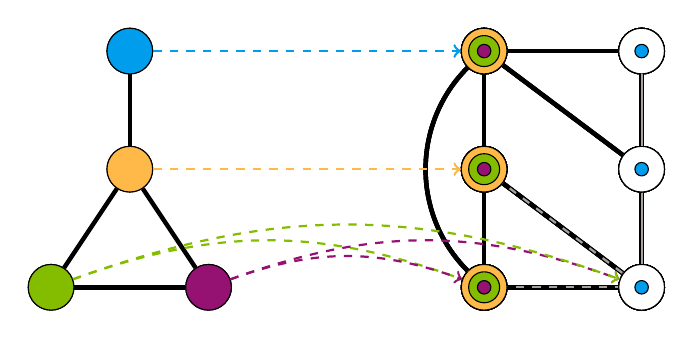
\begin{tikzpicture}
        \node <1> [draw, circle, fill=white, inner sep=4pt, font=\bfseries] (Na) at (1,  0) {\vphantom{1}};
        \node <1> [draw, circle, fill=white, inner sep=4pt, font=\bfseries] (Nb) at (1, -1.5) {\vphantom{1}};
        \node <1> [draw, circle, fill=white, inner sep=4pt, font=\bfseries] (Nc) at (0, -3) {\vphantom{1}};
        \node <1> [draw, circle, fill=white, inner sep=4pt, font=\bfseries] (Nd) at (2, -3) {\vphantom{1}};

        \node <2-> [draw, circle, fill=uofgcobalt, inner sep=4pt, font=\bfseries] (Na) at (1,  0) {\vphantom{1}};
        \node <2-> [draw, circle, fill=uofgpumpkin, inner sep=4pt, font=\bfseries] (Nb) at (1, -1.5) {\vphantom{1}};
        \node <2-> [draw, circle, fill=uofglawn, inner sep=4pt, font=\bfseries] (Nc) at (0, -3) {\vphantom{1}};
        \node <2-> [draw, circle, fill=uofgthistle, inner sep=4pt, font=\bfseries] (Nd) at (2, -3) {\vphantom{1}};

        \draw [ultra thick] (Na) -- (Nb);
        \draw [ultra thick] (Nb) -- (Nc);
        \draw [ultra thick] (Nc) -- (Nd);
        \draw [ultra thick] (Nb) -- (Nd);

        \node <1> [draw, circle, fill=white, inner sep=4pt, font=\bfseries] (N1) at (5.5,  0) {\vphantom{1}};
        \node <1> [draw, circle, fill=white, inner sep=4pt, font=\bfseries] (N2) at (7.5,  0) {\vphantom{1}};
        \node <1> [draw, circle, fill=white, inner sep=4pt, font=\bfseries] (N3) at (5.5, -1.5) {\vphantom{1}};
        \node <1> [draw, circle, fill=white, inner sep=4pt, font=\bfseries] (N4) at (7.5, -1.5) {\vphantom{1}};
        \node <1> [draw, circle, fill=white, inner sep=4pt, font=\bfseries] (N5) at (5.5, -3) {\vphantom{1}};
        \node <1> [draw, circle, fill=white, inner sep=4pt, font=\bfseries] (N6) at (7.5, -3) {\vphantom{1}};

        \node <2> [draw, circle, fill=uofgcobalt, inner sep=4pt, font=\bfseries] (N1) at (5.5,  0) {\vphantom{1}};
        \node <2> [draw, circle, fill=white, inner sep=4pt, font=\bfseries] (N2) at (7.5,  0) {\vphantom{1}};
        \node <2> [draw, circle, fill=uofgpumpkin, inner sep=4pt, font=\bfseries] (N3) at (5.5, -1.5) {\vphantom{1}};
        \node <2> [draw, circle, fill=white, inner sep=4pt, font=\bfseries] (N4) at (7.5, -1.5) {\vphantom{1}};
        \node <2> [draw, circle, fill=uofglawn, inner sep=4pt, font=\bfseries] (N5) at (5.5, -3) {\vphantom{1}};
        \node <2> [draw, circle, fill=uofgthistle, inner sep=4pt, font=\bfseries] (N6) at (7.5, -3) {\vphantom{1}};

        \node <3> [draw, circle, fill=uofgcobalt, inner sep=4pt, font=\bfseries] (N1) at (5.5,  0) {\vphantom{1}};
        \node <3> [draw, circle, fill=white, inner sep=4pt, font=\bfseries] (N2) at (7.5,  0) {\vphantom{1}};
        \node <3> [draw, circle, fill=uofgpumpkin, inner sep=4pt, font=\bfseries] (N3) at (5.5, -1.5) {\vphantom{1}};
        \node <3> [draw, circle, fill=white, inner sep=4pt, font=\bfseries] (N4) at (7.5, -1.5) {\vphantom{1}};
        \node <3> [draw, circle, fill=uofgthistle, inner sep=4pt, font=\bfseries] (N5) at (5.5, -3) {\vphantom{1}};
        \node <3> [draw, circle, fill=uofglawn, inner sep=4pt, font=\bfseries] (N6) at (7.5, -3) {\vphantom{1}};

        \node <4> [draw, circle, fill=uofglawn, inner sep=4pt, font=\bfseries] (N1) at (5.5,  0) {\vphantom{1}};
        \node <4> [draw, circle, fill=uofgthistle, inner sep=1pt, font=\bfseries] (N1b) at (5.5,  0) {\vphantom{1}};
        \node <4> [draw, circle, fill=uofgthistle, inner sep=4pt, font=\bfseries] (N2) at (7.5,  0) {\vphantom{1}};
        \node <4> [draw, circle, fill=uofglawn, inner sep=1pt, font=\bfseries] (N2b) at (7.5,  0) {\vphantom{1}};
        \node <4> [draw, circle, fill=white, inner sep=4pt, font=\bfseries] (N3) at (5.5, -1.5) {\vphantom{1}};
        \node <4> [draw, circle, fill=uofgpumpkin, inner sep=4pt, font=\bfseries] (N4) at (7.5, -1.5) {\vphantom{1}};
        \node <4> [draw, circle, fill=white, inner sep=4pt, font=\bfseries] (N5) at (5.5, -3) {\vphantom{1}};
        \node <4> [draw, circle, fill=uofgcobalt, inner sep=4pt, font=\bfseries] (N6) at (7.5, -3) {\vphantom{1}};

        \node <5> [draw, circle, fill=uofgpumpkin, inner sep=4pt, font=\bfseries] (N1) at (5.5,  0) {\vphantom{1}};
        \node <5> [draw, circle, fill=uofgthistle, inner sep=4pt, font=\bfseries] (N2) at (7.5,  0) {\vphantom{1}};
        \node <5> [draw, circle, fill=uofglawn, inner sep=1pt, font=\bfseries] (N2b) at (7.5,  0) {\vphantom{1}};
        \node <5> [draw, circle, fill=uofgcobalt, inner sep=4pt, font=\bfseries] (N3) at (5.5, -1.5) {\vphantom{1}};
        \node <5> [draw, circle, fill=uofglawn, inner sep=4pt, font=\bfseries] (N4) at (7.5, -1.5) {\vphantom{1}};
        \node <5> [draw, circle, fill=uofgthistle, inner sep=1pt, font=\bfseries] (N4b) at (7.5, -1.5) {\vphantom{1}};
        \node <5> [draw, circle, fill=white, inner sep=4pt, font=\bfseries] (N5) at (5.5, -3) {\vphantom{1}};
        \node <5> [draw, circle, fill=white, inner sep=4pt, font=\bfseries] (N6) at (7.5, -3) {\vphantom{1}};

        \node <6> [draw, circle, fill=white, inner sep=4pt, font=\bfseries] (N1) at (5.5,  0) {\vphantom{1}};
        \node <6> [draw, circle, fill=white, inner sep=4pt, font=\bfseries] (N2) at (7.5,  0) {\vphantom{1}};
        \node <6> [draw, circle, fill=uofgthistle, inner sep=4pt, font=\bfseries] (N3) at (5.5, -1.5) {\vphantom{1}};
        \node <6> [draw, circle, fill=uofglawn, inner sep=1pt, font=\bfseries] (N3b) at (5.5, -1.5) {\vphantom{1}};
        \node <6> [draw, circle, fill=uofgcobalt, inner sep=4pt, font=\bfseries] (N4) at (7.5, -1.5) {\vphantom{1}};
        \node <6> [draw, circle, fill=uofglawn, inner sep=4pt, font=\bfseries] (N5) at (5.5, -3) {\vphantom{1}};
        \node <6> [draw, circle, fill=uofgthistle, inner sep=1pt, font=\bfseries] (N5b) at (5.5, -3) {\vphantom{1}};
        \node <6> [draw, circle, fill=uofgpumpkin, inner sep=4pt, font=\bfseries] (N6) at (7.5, -3) {\vphantom{1}};

        \node <7> [draw, circle, fill=uofgcobalt, inner sep=4pt, font=\bfseries] (N1) at (5.5,  0) {\vphantom{1}};
        \node <7> [draw, circle, fill=white, inner sep=4pt, font=\bfseries] (N2) at (7.5,  0) {\vphantom{1}};
        \node <7> [draw, circle, fill=uofglawn, inner sep=4pt, font=\bfseries] (N3) at (5.5, -1.5) {\vphantom{1}};
        \node <7> [draw, circle, fill=uofgthistle, inner sep=1pt, font=\bfseries] (N3b) at (5.5, -1.5) {\vphantom{1}};
        \node <7> [draw, circle, fill=white, inner sep=4pt, font=\bfseries] (N4) at (7.5, -1.5) {\vphantom{1}};
        \node <7> [draw, circle, fill=uofgpumpkin, inner sep=4pt, font=\bfseries] (N5) at (5.5, -3) {\vphantom{1}};
        \node <7> [draw, circle, fill=uofgthistle, inner sep=4pt, font=\bfseries] (N6) at (7.5, -3) {\vphantom{1}};
        \node <7> [draw, circle, fill=uofglawn, inner sep=1pt, font=\bfseries] (N6b) at (7.5, -3) {\vphantom{1}};

        \node <8> [draw, circle, fill=uofgpumpkin, inner sep=4pt, font=\bfseries] (N1) at (5.5,  0) {\vphantom{1}};
        \node <8> [draw, circle, fill=uofgthistle, inner sep=4pt, font=\bfseries] (N2) at (7.5,  0) {\vphantom{1}};
        \node <8> [draw, circle, fill=uofglawn, inner sep=1pt, font=\bfseries] (N2b) at (7.5,  0) {\vphantom{1}};
        \node <8> [draw, circle, fill=white, inner sep=4pt, font=\bfseries] (N3) at (5.5, -1.5) {\vphantom{1}};
        \node <8> [draw, circle, fill=uofglawn, inner sep=4pt, font=\bfseries] (N4) at (7.5, -1.5) {\vphantom{1}};
        \node <8> [draw, circle, fill=uofgthistle, inner sep=1pt, font=\bfseries] (N4b) at (7.5, -1.5) {\vphantom{1}};
        \node <8> [draw, circle, fill=uofgcobalt, inner sep=4pt, font=\bfseries] (N5) at (5.5, -3) {\vphantom{1}};
        \node <8> [draw, circle, fill=white, inner sep=4pt, font=\bfseries] (N6) at (7.5, -3) {\vphantom{1}};

        \node <9> [draw, circle, fill=uofgpumpkin, inner sep=4pt, font=\bfseries] (N1) at (5.5,  0) {\vphantom{1}};
        \node <9> [draw, circle, fill=uofglawn, inner sep=2pt, font=\bfseries] (N1b) at (5.5,  0) {\vphantom{1}};
        \node <9> [draw, circle, fill=uofgthistle, inner sep=-1pt, font=\bfseries] (N1c) at (5.5,  0) {\vphantom{1}};
        \node <9> [draw, circle, fill=white, inner sep=4pt, font=\bfseries] (N2) at (7.5,  0) {\vphantom{1}};
        \node <9> [draw, circle, fill=uofgcobalt, inner sep=-1pt, font=\bfseries] (N2b) at (7.5,  0) {\vphantom{1}};
        \node <9> [draw, circle, fill=uofgpumpkin, inner sep=4pt, font=\bfseries] (N3) at (5.5, -1.5) {\vphantom{1}};
        \node <9> [draw, circle, fill=uofglawn, inner sep=2pt, font=\bfseries] (N3b) at (5.5, -1.5) {\vphantom{1}};
        \node <9> [draw, circle, fill=uofgthistle, inner sep=-1pt, font=\bfseries] (N3c) at (5.5, -1.5) {\vphantom{1}};
        \node <9> [draw, circle, fill=white, inner sep=4pt, font=\bfseries] (N4) at (7.5, -1.5) {\vphantom{1}};
        \node <9> [draw, circle, fill=uofgcobalt, inner sep=-1pt, font=\bfseries] (N4b) at (7.5, -1.5) {\vphantom{1}};
        \node <9> [draw, circle, fill=uofgpumpkin, inner sep=4pt, font=\bfseries] (N5) at (5.5, -3) {\vphantom{1}};
        \node <9> [draw, circle, fill=uofglawn, inner sep=2pt, font=\bfseries] (N5b) at (5.5, -3) {\vphantom{1}};
        \node <9> [draw, circle, fill=uofgthistle, inner sep=-1pt, font=\bfseries] (N5c) at (5.5, -3) {\vphantom{1}};
        \node <9> [draw, circle, fill=white, inner sep=4pt, font=\bfseries] (N6) at (7.5, -3) {\vphantom{1}};
        \node <9> [draw, circle, fill=uofgcobalt, inner sep=-1pt, font=\bfseries] (N6b) at (7.5, -3) {\vphantom{1}};

        \draw <1> [thick, color=uofgsandstone!50] (N1) -- (N2);
        \draw <1> [thick, color=uofgsandstone!50] (N1) -- (N3);
        \draw <1> [thick, color=uofgsandstone!50] (N1) -- (N4);
        \draw <1> [thick, color=uofgsandstone!50] (N2) -- (N4);
        \draw <1> [thick, color=uofgsandstone!50] (N3) -- (N5);
        \draw <1> [thick, color=uofgsandstone!50] (N3) -- (N6);
        \draw <1> [thick, color=uofgsandstone!50] (N4) -- (N6);
        \draw <1> [thick, color=uofgsandstone!50] (N5) -- (N6);
        \draw <1> [thick, color=uofgsandstone!50] (N1) to [in=135, out=225] (N5);

        \draw <2-3> [thick, color=uofgsandstone!50] (N1) -- (N2);
        \draw <2-3> [ultra thick] (N1) -- (N3);
        \draw <2-3> [thick, color=uofgsandstone!50] (N1) -- (N4);
        \draw <2-3> [thick, color=uofgsandstone!50] (N2) -- (N4);
        \draw <2-3> [ultra thick] (N3) -- (N5);
        \draw <2-3> [ultra thick] (N3) -- (N6);
        \draw <2-3> [thick, color=uofgsandstone!50] (N4) -- (N6);
        \draw <2-3> [ultra thick] (N5) -- (N6);
        \draw <2-3> [thick, color=uofgsandstone!50] (N1) to [in=135, out=225] (N5);

        \draw <4> [ultra thick] (N1) -- (N2);
        \draw <4> [thick, color=uofgsandstone!50] (N1) -- (N3);
        \draw <4> [ultra thick] (N1) -- (N4);
        \draw <4> [ultra thick] (N2) -- (N4);
        \draw <4> [thick, color=uofgsandstone!50] (N3) -- (N5);
        \draw <4> [thick, color=uofgsandstone!50] (N3) -- (N6);
        \draw <4> [ultra thick] (N4) -- (N6);
        \draw <4> [thick, color=uofgsandstone!50] (N5) -- (N6);
        \draw <4> [thick, color=uofgsandstone!50] (N1) to [in=135, out=225] (N5);

        \draw <5> [ultra thick] (N1) -- (N2);
        \draw <5> [ultra thick] (N1) -- (N3);
        \draw <5> [ultra thick] (N1) -- (N4);
        \draw <5> [ultra thick] (N2) -- (N4);
        \draw <5> [thick, color=uofgsandstone!50] (N3) -- (N5);
        \draw <5> [thick, color=uofgsandstone!50] (N3) -- (N6);
        \draw <5> [thick, color=uofgsandstone!50] (N4) -- (N6);
        \draw <5> [thick, color=uofgsandstone!50] (N5) -- (N6);
        \draw <5> [thick, color=uofgsandstone!50] (N1) to [in=135, out=225] (N5);

        \draw <6> [thick, color=uofgsandstone!50] (N1) -- (N2);
        \draw <6> [thick, color=uofgsandstone!50] (N1) -- (N3);
        \draw <6> [thick, color=uofgsandstone!50] (N1) -- (N4);
        \draw <6> [thick, color=uofgsandstone!50] (N2) -- (N4);
        \draw <6> [ultra thick] (N3) -- (N5);
        \draw <6> [ultra thick] (N3) -- (N6);
        \draw <6> [ultra thick] (N4) -- (N6);
        \draw <6> [ultra thick] (N5) -- (N6);
        \draw <6> [thick, color=uofgsandstone!50] (N1) to [in=135, out=225] (N5);

        \draw <7> [thick, color=uofgsandstone!50] (N1) -- (N2);
        \draw <7> [thick, color=uofgsandstone!50] (N1) -- (N3);
        \draw <7> [thick, color=uofgsandstone!50] (N1) -- (N4);
        \draw <7> [thick, color=uofgsandstone!50] (N2) -- (N4);
        \draw <7> [ultra thick] (N3) -- (N5);
        \draw <7> [ultra thick] (N3) -- (N6);
        \draw <7> [thick, color=uofgsandstone!50] (N4) -- (N6);
        \draw <7> [ultra thick] (N5) -- (N6);
        \draw <7> [ultra thick] (N1) to [in=135, out=225] (N5);

        \draw <8> [ultra thick] (N1) -- (N2);
        \draw <8> [thick, color=uofgsandstone!50] (N1) -- (N3);
        \draw <8> [ultra thick] (N1) -- (N4);
        \draw <8> [ultra thick] (N2) -- (N4);
        \draw <8> [thick, color=uofgsandstone!50] (N3) -- (N5);
        \draw <8> [thick, color=uofgsandstone!50] (N3) -- (N6);
        \draw <8> [thick, color=uofgsandstone!50] (N4) -- (N6);
        \draw <8> [thick, color=uofgsandstone!50] (N5) -- (N6);
        \draw <8> [ultra thick] (N1) to [in=135, out=225] (N5);

        \draw <9> [ultra thick, dashed] (N1) -- (N2);
        \draw <9> [ultra thick] (N1) -- (N3);
        \draw <9> [ultra thick, dashed] (N1) -- (N4);
        \draw <9> [thick, color=uofgsandstone!50] (N2) -- (N4);
        \draw <9> [ultra thick] (N3) -- (N5);
        \draw <9> [ultra thick, dashed] (N3) -- (N6);
        \draw <9> [thick, color=uofgsandstone!50] (N4) -- (N6);
        \draw <9> [ultra thick, dashed] (N5) -- (N6);
        \draw <9> [ultra thick] (N1) to [in=135, out=225] (N5);

        \draw <2> [thick, dashed, color=uofgcobalt, arrows=->] (Na) to (N1);
        \draw <2> [thick, dashed, color=uofgpumpkin, arrows=->] (Nb) to (N3);
        \draw <2> [thick, dashed, color=uofglawn, arrows=->] (Nc) to [out=20, in=160] (N5);
        \draw <2> [thick, dashed, color=uofgthistle, arrows=->] (Nd) to [out=20, in=160] (N6);

        \draw <3> [thick, dashed, color=uofgcobalt, arrows=->] (Na) to (N1);
        \draw <3> [thick, dashed, color=uofgpumpkin, arrows=->] (Nb) to (N3);
        \draw <3> [thick, dashed, color=uofglawn, arrows=->] (Nc) to [out=20, in=160] (N6);
        \draw <3> [thick, dashed, color=uofgthistle, arrows=->] (Nd) to [out=20, in=160] (N5);
    \end{tikzpicture}

\begin{itemize}
    \item Find the \emph{pattern} inside the \emph{target}.
    \item Applications in compilers, biochemistry, model checking, pattern recognition, \ldots
    \item <3-> Often want to find \emph{all} matches.
\end{itemize}
\end{frame}

\begin{frame}{The Maximum Clique Problem}
    \begin{center}
    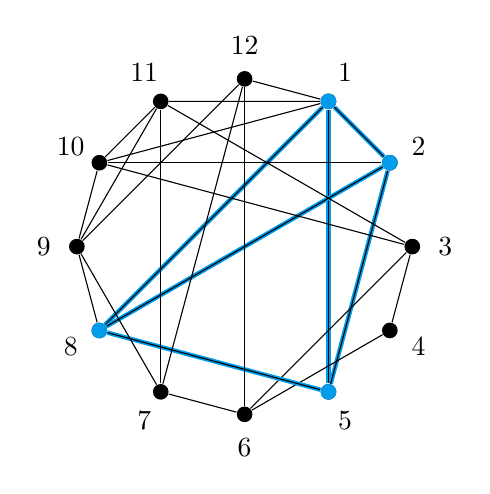
\begin{tikzpicture}
        \begin{scope}[scale=1.5]
        \newcount \myc
        \foreach \n in {3, 4, 6, 7, 9, 10, 11, 12}{
            \myc=\n \advance\myc by -1 \multiply\myc by -360 \divide\myc by 12 \advance\myc by 60.0
            \node[anchor=center] (L\n) at (\the\myc:1.7) {\n};
            \node[anchor=center, circle, fill=black, inner sep=2pt] (N\n) at (\the\myc:1.42) {};
        }
        \foreach \n in {1, 2, 5, 8}{
            \myc=\n \advance\myc by -1 \multiply\myc by -360 \divide\myc by 12 \advance\myc by 60.0
            \node[anchor=center] (L\n) at (\the\myc:1.7) {\n};
            \node<1>[anchor=center, circle, fill=black, inner sep=2pt] (N\n) at (\the\myc:1.42) {};
            \node<2>[anchor=center, circle, fill=uofgcobalt, inner sep=2pt] (N\n) at (\the\myc:1.42) {};
        }
        \draw <2> [ultra thick, color=uofgcobalt] (N1) -- (N2);
        \draw <2> [ultra thick, color=uofgcobalt] (N1) -- (N5);
        \draw <2> [ultra thick, color=uofgcobalt] (N1) -- (N8);
        \draw <1> (N1) -- (N2);
        \draw <1> (N1) -- (N5);
        \draw <1> (N1) -- (N8);
        \draw (N1) -- (N10);
        \draw (N1) -- (N11);
        \draw (N1) -- (N12);
        \draw <2> [ultra thick, color=uofgcobalt] (N2) -- (N5);
        \draw <2> [ultra thick, color=uofgcobalt] (N2) -- (N8);
        \draw <1> (N2) -- (N5);
        \draw <1> (N2) -- (N8);
        \draw (N2) -- (N10);
        \draw (N3) -- (N4);
        \draw (N3) -- (N6);
        \draw (N3) -- (N10);
        \draw (N3) -- (N11);
        \draw (N4) -- (N6);
        \draw <2> [ultra thick, color=uofgcobalt] (N5) -- (N8);
        \draw <1> (N5) -- (N8);
        \draw (N6) -- (N7);
        \draw (N6) -- (N12);
        \draw (N7) -- (N9);
        \draw (N7) -- (N11);
        \draw (N7) -- (N12);
        \draw (N8) -- (N9);
        \draw (N9) -- (N10);
        \draw (N9) -- (N11);
        \draw (N9) -- (N12);
        \draw (N10) -- (N11);
    \end{scope}
    \end{tikzpicture}
\end{center}
\end{frame}

\section{CP Helps Us Understand Algorithms}

\begin{frame}{Understanding Colour Ordering}
    \only<1>{
        \centering
    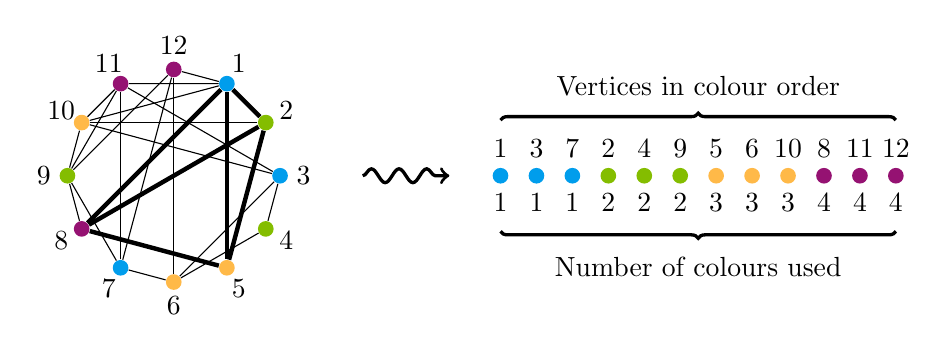
\begin{tikzpicture}
        \begin{scope}[scale=1.5]
        \newcount \myc
        \foreach \n in {1, 3, 7}{
            \myc=\n \advance\myc by -1 \multiply\myc by -360 \divide\myc by 12 \advance\myc by 60.0
            \node[anchor=center] (L\n) at (\the\myc:1.1) {\n};
            \node[anchor=center, circle, fill=uofgcobalt, inner sep=2pt] (N\n) at (\the\myc:0.9) {};
        }
        \foreach \n in {2, 4, 9}{
            \myc=\n \advance\myc by -1 \multiply\myc by -360 \divide\myc by 12 \advance\myc by 60.0
            \node[anchor=center] (l\n) at (\the\myc:1.1) {\n};
            \node[anchor=center, circle, fill=uofglawn, inner sep=2pt] (N\n) at (\the\myc:0.9) {};
        }
        \foreach \n in {5, 6, 10}{
            \myc=\n \advance\myc by -1 \multiply\myc by -360 \divide\myc by 12 \advance\myc by 60.0
            \node[anchor=center] (L\n) at (\the\myc:1.1) {\n};
            \node[anchor=center, circle, fill=uofgpumpkin, inner sep=2pt] (N\n) at (\the\myc:0.9) {};
        }
        \foreach \n in {8, 11, 12}{
            \myc=\n \advance\myc by -1 \multiply\myc by -360 \divide\myc by 12 \advance\myc by 60.0
            \node[anchor=center] (L\n) at (\the\myc:1.1) {\n};
            \node[anchor=center, circle, fill=uofgthistle, inner sep=2pt] (N\n) at (\the\myc:0.9) {};
        }
        \draw [ultra thick] (N1) -- (N2);
        \draw [ultra thick] (N1) -- (N5);
        \draw [ultra thick] (N1) -- (N8);
        \draw (N1) -- (N10);
        \draw (N1) -- (N11);
        \draw (N1) -- (N12);
        \draw [ultra thick] (N2) -- (N5);
        \draw [ultra thick] (N2) -- (N8);
        \draw (N2) -- (N10);
        \draw (N3) -- (N4);
        \draw (N3) -- (N6);
        \draw (N3) -- (N10);
        \draw (N3) -- (N11);
        \draw (N4) -- (N6);
        \draw [ultra thick] (N5) -- (N8);
        \draw (N6) -- (N7);
        \draw (N6) -- (N12);
        \draw (N7) -- (N9);
        \draw (N7) -- (N11);
        \draw (N7) -- (N12);
        \draw (N8) -- (N9);
        \draw (N9) -- (N10);
        \draw (N9) -- (N11);
        \draw (N9) -- (N12);
        \draw (N10) -- (N11);
    \end{scope}

\draw [processarrow] (2.4, 0) -> (3.5, 0);

\coordinate (Ms) at (3.8, 0.0);
\node[right = 0.35 of Ms,  anchor=center, circle, fill=uofgcobalt,  inner sep=2pt] (V1) {};
\node[right = 0.35 of V1,  anchor=center, circle, fill=uofgcobalt,  inner sep=2pt] (V2) {};
\node[right = 0.35 of V2,  anchor=center, circle, fill=uofgcobalt,  inner sep=2pt] (V3) {};
\node[right = 0.35 of V3,  anchor=center, circle, fill=uofglawn,    inner sep=2pt] (V4) {};
\node[right = 0.35 of V4,  anchor=center, circle, fill=uofglawn,    inner sep=2pt] (V5) {};
\node[right = 0.35 of V5,  anchor=center, circle, fill=uofglawn,    inner sep=2pt] (V6) {};
\node[right = 0.35 of V6,  anchor=center, circle, fill=uofgpumpkin, inner sep=2pt] (V7) {};
\node[right = 0.35 of V7,  anchor=center, circle, fill=uofgpumpkin, inner sep=2pt] (V8) {};
\node[right = 0.35 of V8,  anchor=center, circle, fill=uofgpumpkin, inner sep=2pt] (V9) {};
\node[right = 0.35 of V9,  anchor=center, circle, fill=uofgthistle, inner sep=2pt] (V10) {};
\node[right = 0.35 of V10, anchor=center, circle, fill=uofgthistle, inner sep=2pt] (V11) {};
\node[right = 0.35 of V11, anchor=center, circle, fill=uofgthistle, inner sep=2pt] (V12) {};
\node[above = 0.0 of V1] {1};
\node[above = 0.0 of V2] {3};
\node[above = 0.0 of V3] {7};
\node[above = 0.0 of V4] {2};
\node[above = 0.0 of V5] {4};
\node[above = 0.0 of V6] {9};
\node[above = 0.0 of V7] {5};
\node[above = 0.0 of V8] {6};
\node[above = 0.0 of V9] {10};
\node[above = 0.0 of V10] {8};
\node[above = 0.0 of V11] {11};
\node[above = 0.0 of V12] {12};
\node[below = 0.0 of V1] {1};
\node[below = 0.0 of V2] {1};
\node[below = 0.0 of V3] {1};
\node[below = 0.0 of V4] {2};
\node[below = 0.0 of V5] {2};
\node[below = 0.0 of V6] {2};
\node[below = 0.0 of V7] {3};
\node[below = 0.0 of V8] {3};
\node[below = 0.0 of V9] {3};
\node[below = 0.0 of V10] {4};
\node[below = 0.0 of V11] {4};
\node[below = 0.0 of V12] {4};

\draw[brace] ($(V1.north)+(0.0,0.6)$) -- ($(V12.north)+(0.0,0.6)$);
\node[anchor=south] at ($(V1)!0.5!(V12)$)[yshift=0.9cm] { Vertices in colour order };

\draw[brace] ($(V12.south)+(0.0,-0.6)$) -- ($(V1.south)+(0.0,-0.6)$);
\node[anchor=south] at ($(V1)!0.5!(V12)$)[yshift=-1.4cm] { Number of colours used };

    \end{tikzpicture}
    }\only<2->{
    \begin{itemize}
        \item Vertices in the rightmost colour class are ``generally expected [to have a] high
            probability of belonging to a maximum clique'' according to Tomita and Kameda, J. Global
            Optimization, 37(1) 2007.
        \item <3-> It's not true.
        \item <4-> Right to left is still better even if the algorithm is only proving optimality.
        \item <4-> Better clique algorithms have \emph{worse} anytime behaviour and take
            \emph{longer} to find a strong incumbent.
        \item <5-> Rethinking the algorithms in terms of constraint programming variables and
            heuristics explains this.
    \end{itemize}}
\end{frame}

\begin{frame}{Weights and Search Orders}
    \begin{itemize}
        \item Lack of good benchmark instances for the maximum weight clique problem.
            \begin{itemize}
                \item Many practical applications, but the instances aren't easily available.
            \end{itemize}
        \item Take the DIMACS clique instances, and give vertex $i$ weight $i \operatorname{mod} 200 + 1$.
        \item <2-> Puts a huge emphasis on weights and very little on graph structure.
        \item <2-> Real instances have much more interesting relationships.
        \item <3-> Need search heuristics which consider both weight and adjacency, but you'd never find
            this out on the usual benchmarks.
    \end{itemize}
\end{frame}

\begin{frame}{Do Labels Make Things Easier or Harder?}

    \begin{center}
    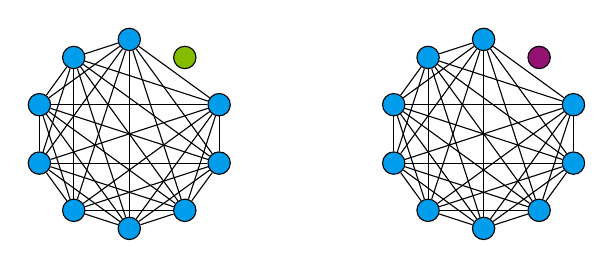
\begin{tikzpicture}[scale=0.5,every node/.style={font=\footnotesize}]
        \begin{scope}
            \newcount \myc
            \newcount \myd
            \newcount \mye
            \foreach \n in {1, ..., 9}{
                \myc=\n \advance\myc by -1 \multiply\myc by -360 \divide\myc by 10 \advance\myc by 18.0
                \node[draw, circle, fill=uofgcobalt, inner sep=0.5pt] (N\n) at (\the\myc:2.4) {\phantom{0}};
            }
            \node[draw, circle, fill=uofglawn, inner sep=0.5pt] (N10) at (54.0:2.4) {\phantom{0}};

            \foreach \n in {1, ..., 8}{
                \myd=\n
                \myc=\n \advance\myc by 1
                \foreach \m in {\the\myc, ..., 9}{
                    \mye=\m
                    \draw (N\the\myd) -- (N\the\mye);
                }
            }
        \end{scope}
        \begin{scope}[xshift=9cm]
            \newcount \myc
            \newcount \myd
            \newcount \mye
            \foreach \n in {1, ..., 9}{
                \myc=\n \advance\myc by -1 \multiply\myc by -360 \divide\myc by 10 \advance\myc by 18.0
                \node[draw, circle, fill=uofgcobalt, inner sep=0.5pt] (N\n) at (\the\myc:2.4) {\phantom{0}};
            }
            \node[draw, circle, fill=uofgthistle, inner sep=0.5pt] (N10) at (54.0:2.4) {\phantom{0}};

            \foreach \n in {1, ..., 8}{
                \myd=\n
                \myc=\n \advance\myc by 1
                \foreach \m in {\the\myc, ..., 9}{
                    \mye=\m
                    \draw (N\the\myd) -- (N\the\mye);
                }
            }
        \end{scope}
    \end{tikzpicture}
    \end{center}

    \bigskip

    \begin{itemize}
        \item <2-> Whole research area based around detecting unsatisfiability to avoid having to call a subgraph
            isomorphism solver.
        \item <2-> ``Subgraph isomorphism is NP-complete, so anything we can do to avoid doing a subgraph query
            is going to speed things up.''
    \end{itemize}
\end{frame}

\section{Using CP to Improve Subgraph Algorithms}

\begin{frame}{Search, Restarts, and Nogoods}
    \only<1>{
    \begin{itemize}
        \item We know that vanilla backtracking search isn't great.
        \item The same is true in subgraph solving:
            \begin{itemize}
                \item Slightly-random value-ordering heuristic.
                \item Aggressive restarts.
                \item Nogood recording.
            \end{itemize}
        \item Two orders of magnitude speedup on satisfiable instances, without affecting unsatisfiable
            performance.
    \end{itemize}}\only<2>{
    \centering\includegraphics{gen-graph-sbs.pdf}
}
\end{frame}

\begin{frame}{Parallel Search, for (Nearly) Free}
    \only<1>{
    \begin{itemize}
        \item Give each thread a different seed for the slightly-random value-ordering heuristic.
        \item Share nogoods on restarts.
        \item 24 times speedup on 36 shared memory cores, 145 times speedup on 720 distributed cores.
    \end{itemize}}%
\only<2>{
    \centering\includegraphics{gen-graph-dist.pdf}
}
\end{frame}

\begin{frame}{Why Isn't Anyone Else Doing This?}
    \begin{itemize}
        \item They don't know it can be done.
        \item Implementation isn't easy.
    \end{itemize}
\end{frame}

\begin{frame}{Symmetries}
    \begin{itemize}
        \item The CP community understands symmetries much better than most algorithm implementers.
        \item Huge potential for speedups in subgraph solving.
        \item <2-> But a robust implementation is hard.
    \end{itemize}
\end{frame}

\begin{frame}{Counting and Sampling}
    \begin{itemize}
        \item People don't want to enumerate subgraph matches, they want an approximate count or
            a uniform sample.
        \item We know how to do this for SAT and CP.
        \item <2-> But a robust implementation is hard.
    \end{itemize}
\end{frame}

\begin{frame}{Motivation}
    Potentially huge gains to be had from making CP techniques easily
    deployable and robust in non-CP settings.
\end{frame}

\section{Stealing From SAT to Improve CP}

\begin{frame}{Demotivation}
    My first experience of research: a summer internship reimplementing a clique enumeration algorithm from the literature.

    \bigskip

    My code produced the ``wrong'' answer on a few instances.

    \bigskip\pause

    I spent a month trying to find and fix it.

    \bigskip\pause

    The published answers were wrong.
\end{frame}

\begin{frame}{This is an Ongoing Problem}
    \begin{itemize}
        \item When you solve a billion problem instances, things have to work reliably.
        \item For clique solving: 0.1\% of ``solved'' instances gave suboptimal answers.
        \item For subgraph solving: crashes, missing solutions, infeasible solutions.
    \end{itemize}
\end{frame}

\begin{frame}{The Slide That Gets Me Into Trouble}
    \begin{itemize}
        \item 2021 MiniZinc Challenge: for 1.28\% of ``solved'' instances, we get the wrong solution.
            \begin{itemize}
                \item False claims of unsatisfiability.
                \item False claims of optimality.
                \item Infeasible solutions produced.
            \end{itemize}
        \item This includes academic and commercial CP and MIP solvers.
            \begin{itemize}
                \item Gurobi run on the same instance on the same hardware twice in a row
                    can claim both unsatisfiability and incorrect optimality.
            \end{itemize}
        \item <2-> Extensive testing hasn't fixed this.
        \item <2-> Formal methods are far from being able to handle solvers.
        \item <3-> The SAT community has largely solved this problem.
    \end{itemize}
\end{frame}

\begin{frame}{Proof Logging}
    \vspace*{-1.0em}
    \begin{center}
        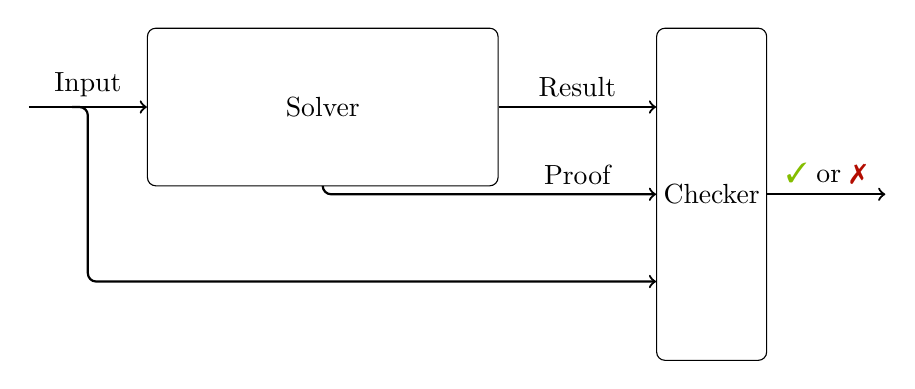
\begin{tikzpicture}
            \node (solver) [%
            inner xsep=5em,
            inner ysep=2.5em, 
            draw, rounded corners=3pt] { Solver };

            \node (checker) [%
            right=2cm of solver.north east, 
            anchor=north west,
            inner xsep=0.25em,
            draw, rounded corners=3pt, 
            minimum height=12em, 
            visible on=<3->] { Checker };

            \draw [->, thick] (solver.east) -- (solver.east -| checker.west)
                coordinate [midway] (solutionmid) node [above, midway]
                { 
                  Result
                };

            \draw [->, thick, rounded corners=3pt, visible on=<2->] (solver.south) -- (solver.south |- checker.west)
                -- (checker.west) coordinate [midway] (proofmid);

            \coordinate (prooflabel) at (proofmid-|solutionmid);
            \node [above=0cm of prooflabel, visible on=<2->] { Proof };

            \coordinate [right=1.5cm of checker.east] (verified);
            \draw [->, thick, visible on=<4->] (checker.east) -- (verified) node [above, midway] { \textcolor{uofglawn}{\ding{51}} or \textcolor{uofgpillarbox}{\ding{55}} };

            \coordinate [left=1.5cm of solver.west] (input);
            \draw [->, thick] (input) -- (solver.west) coordinate [midway] (inputmid) node [above, midway] { Input };

            \coordinate (checkerbotleft) at ($(checker.west)+($(checker.west)-(solver.east-|checker.west)$)$);

            \draw [->, thick, rounded corners=3pt, visible on=<3->] ($(inputmid)+(-0.2,0)$) -- (inputmid) -- (inputmid |- checkerbotleft) -- (checkerbotleft);
        \end{tikzpicture}
      \end{center}
    \vspace*{-0.7em}
  \begin{enumerate}
  \item<1->
    Run solver on problem input.
  \item<2->
    Get both a solution and a proof as output.
  \item<3->
    Feed input + solution + proof to proof checker.
  \item<4->
    Verify that proof checker says solution is correct.
  \end{enumerate}
\end{frame}

\begin{frame}{We Can't just Steal SAT Proof Logging}
    \only<1>{\begin{itemize}
        \item Need to be able to reason about 400+ global constraints.
        \item SAT proof checking struggles with parity and cardinality reasoning.
            \begin{itemize}
                \item Both theoretical and practical limitations.
                \item All-different requires exponential length proofs in resolution.
            \end{itemize}
        \item Need to deal with optimisation, enumeration, \ldots
            \begin{itemize}
                \item Did that clique graph have a 5-clique we didn't spot?
                \item Did we really find all the subgraph matches?
            \end{itemize}
    \end{itemize}}
    \only<2>{
    \begin{itemize}
        \item Do we need a proof format that knows about every single propagation algorithm?
        \item Would you trust a proof checker for such a format?
    \end{itemize}}
\end{frame}

\begin{frame}{The Remarkable Claim}
    \begin{itemize}
        \item If we move from CNF to 0/1 integer linear inequalities, and from resolution
            to cutting planes, we can efficiently justify strong reasoning in a very simple
            proof format.

            \pause

        \item Do all of your solving using a powerful solver, as normal.
        \item Have the solver output \emph{justifications} in a simpler format.
    \end{itemize}
\end{frame}

\begin{frame}{This Actually Works}
    \begin{itemize}
        \item So far:
            \begin{itemize}
                \item Clique and weighted clique.
                \item Subgraph isomorphism, including degree reasoning, paths reasoning.
                \item Maximum common connected subgraph, including microstructure reformulation.
            \end{itemize}
        \item Ongoing work on CP:
            \begin{itemize}
                \item Integer linear (in)equalities, including with large domains.
                \item All different.
                \item Table, Regular, Smart Table.
                \item Circuit.
                \item Element, Min, Max.
            \end{itemize}
        \item Our proof system doesn't need to know what graphs or integer variables are.
    \end{itemize}
\end{frame}

\begin{frame}{But Wait, There's More!}
    \begin{itemize}
        \item We can verify reasoning about symmetries:
            \begin{itemize}
                \item Find your symmetries however you want.
                \item Add breaking constraints, and output simple justifications.
            \end{itemize}
        \item The proof checker doesn't know what a symmetry is, and doesn't know
            any group theory.
        \item Also works for dominance.
    \end{itemize}
\end{frame}

\begin{frame}{Proof Logging Makes Solver Implementation Easier}
    \begin{itemize}
        \item I implemented a solver, with ``trust me'' assertions for linear inequalities.
        \item It was producing the right answer on all of the tests.
        \item I added proof logging for linear inequalities. Many of the proofs failed.
            \begin{itemize}
                \item Integer div and mod on negative numbers in C++ is weird.
                \item I had forgotten this.
            \end{itemize}
        \item Ongoing experience as we add constraints: proof logging is consistently finding edge cases
            that testing misses.
        \item Proof logging is less effort and less code than writing good tests.
    \end{itemize}
\end{frame}

\begin{frame}{Proof Logs for Empirical Algorithmics?}
    \begin{itemize}
        \item Can we analyse proof logs to understand why solvers work so well?
    \end{itemize}
\end{frame}

\begin{frame}{Getting Started}
    Tutorial slides and video: \\
        \qquad\url{https://ciaranm.github.io/}

    \bigskip

    Solvers: \\
        \qquad\url{https://github.com/ciaranm/glasgow-constraint-solver} \\
        \qquad\url{https://github.com/ciaranm/glasgow-subgraph-solver}

    \bigskip

    Proof checker: \\
        \qquad\url{https://gitlab.com/MIAOresearch/software/VeriPB}
\end{frame}

\begin{frame}{The Big Question}

    \begin{center}
    {\huge Why does this work?}
    \end{center}

    \bigskip

    \uncover<2->{
    \begin{itemize}
        \item Justifying facts seems to be easier than finding facts.
        \item Need to be able to combine lookahead, counting, logical
            reasoning, linear relaxations, and ``without loss of generality''.
        \item Does your favourite propagator do more than this?
    \end{itemize}}
\end{frame}

\begin{frame}{Auditable Solving}
    \begin{itemize}
        \item ``The Algorithm'' is making a decision that affects your life or livelihood.
        \item We could take a human-understandable description of the problem,
            and provide an auditable record that the correct solution was reached by
            legitimate means.
        \item Probably useful even if the problems aren't that hard.
    \end{itemize}
\end{frame}

{
    \usebackgroundtemplate{
        \tikz[overlay, remember picture]
        \node[at=(current page.south), anchor=south, yshift=-1cm, inner sep=0pt]{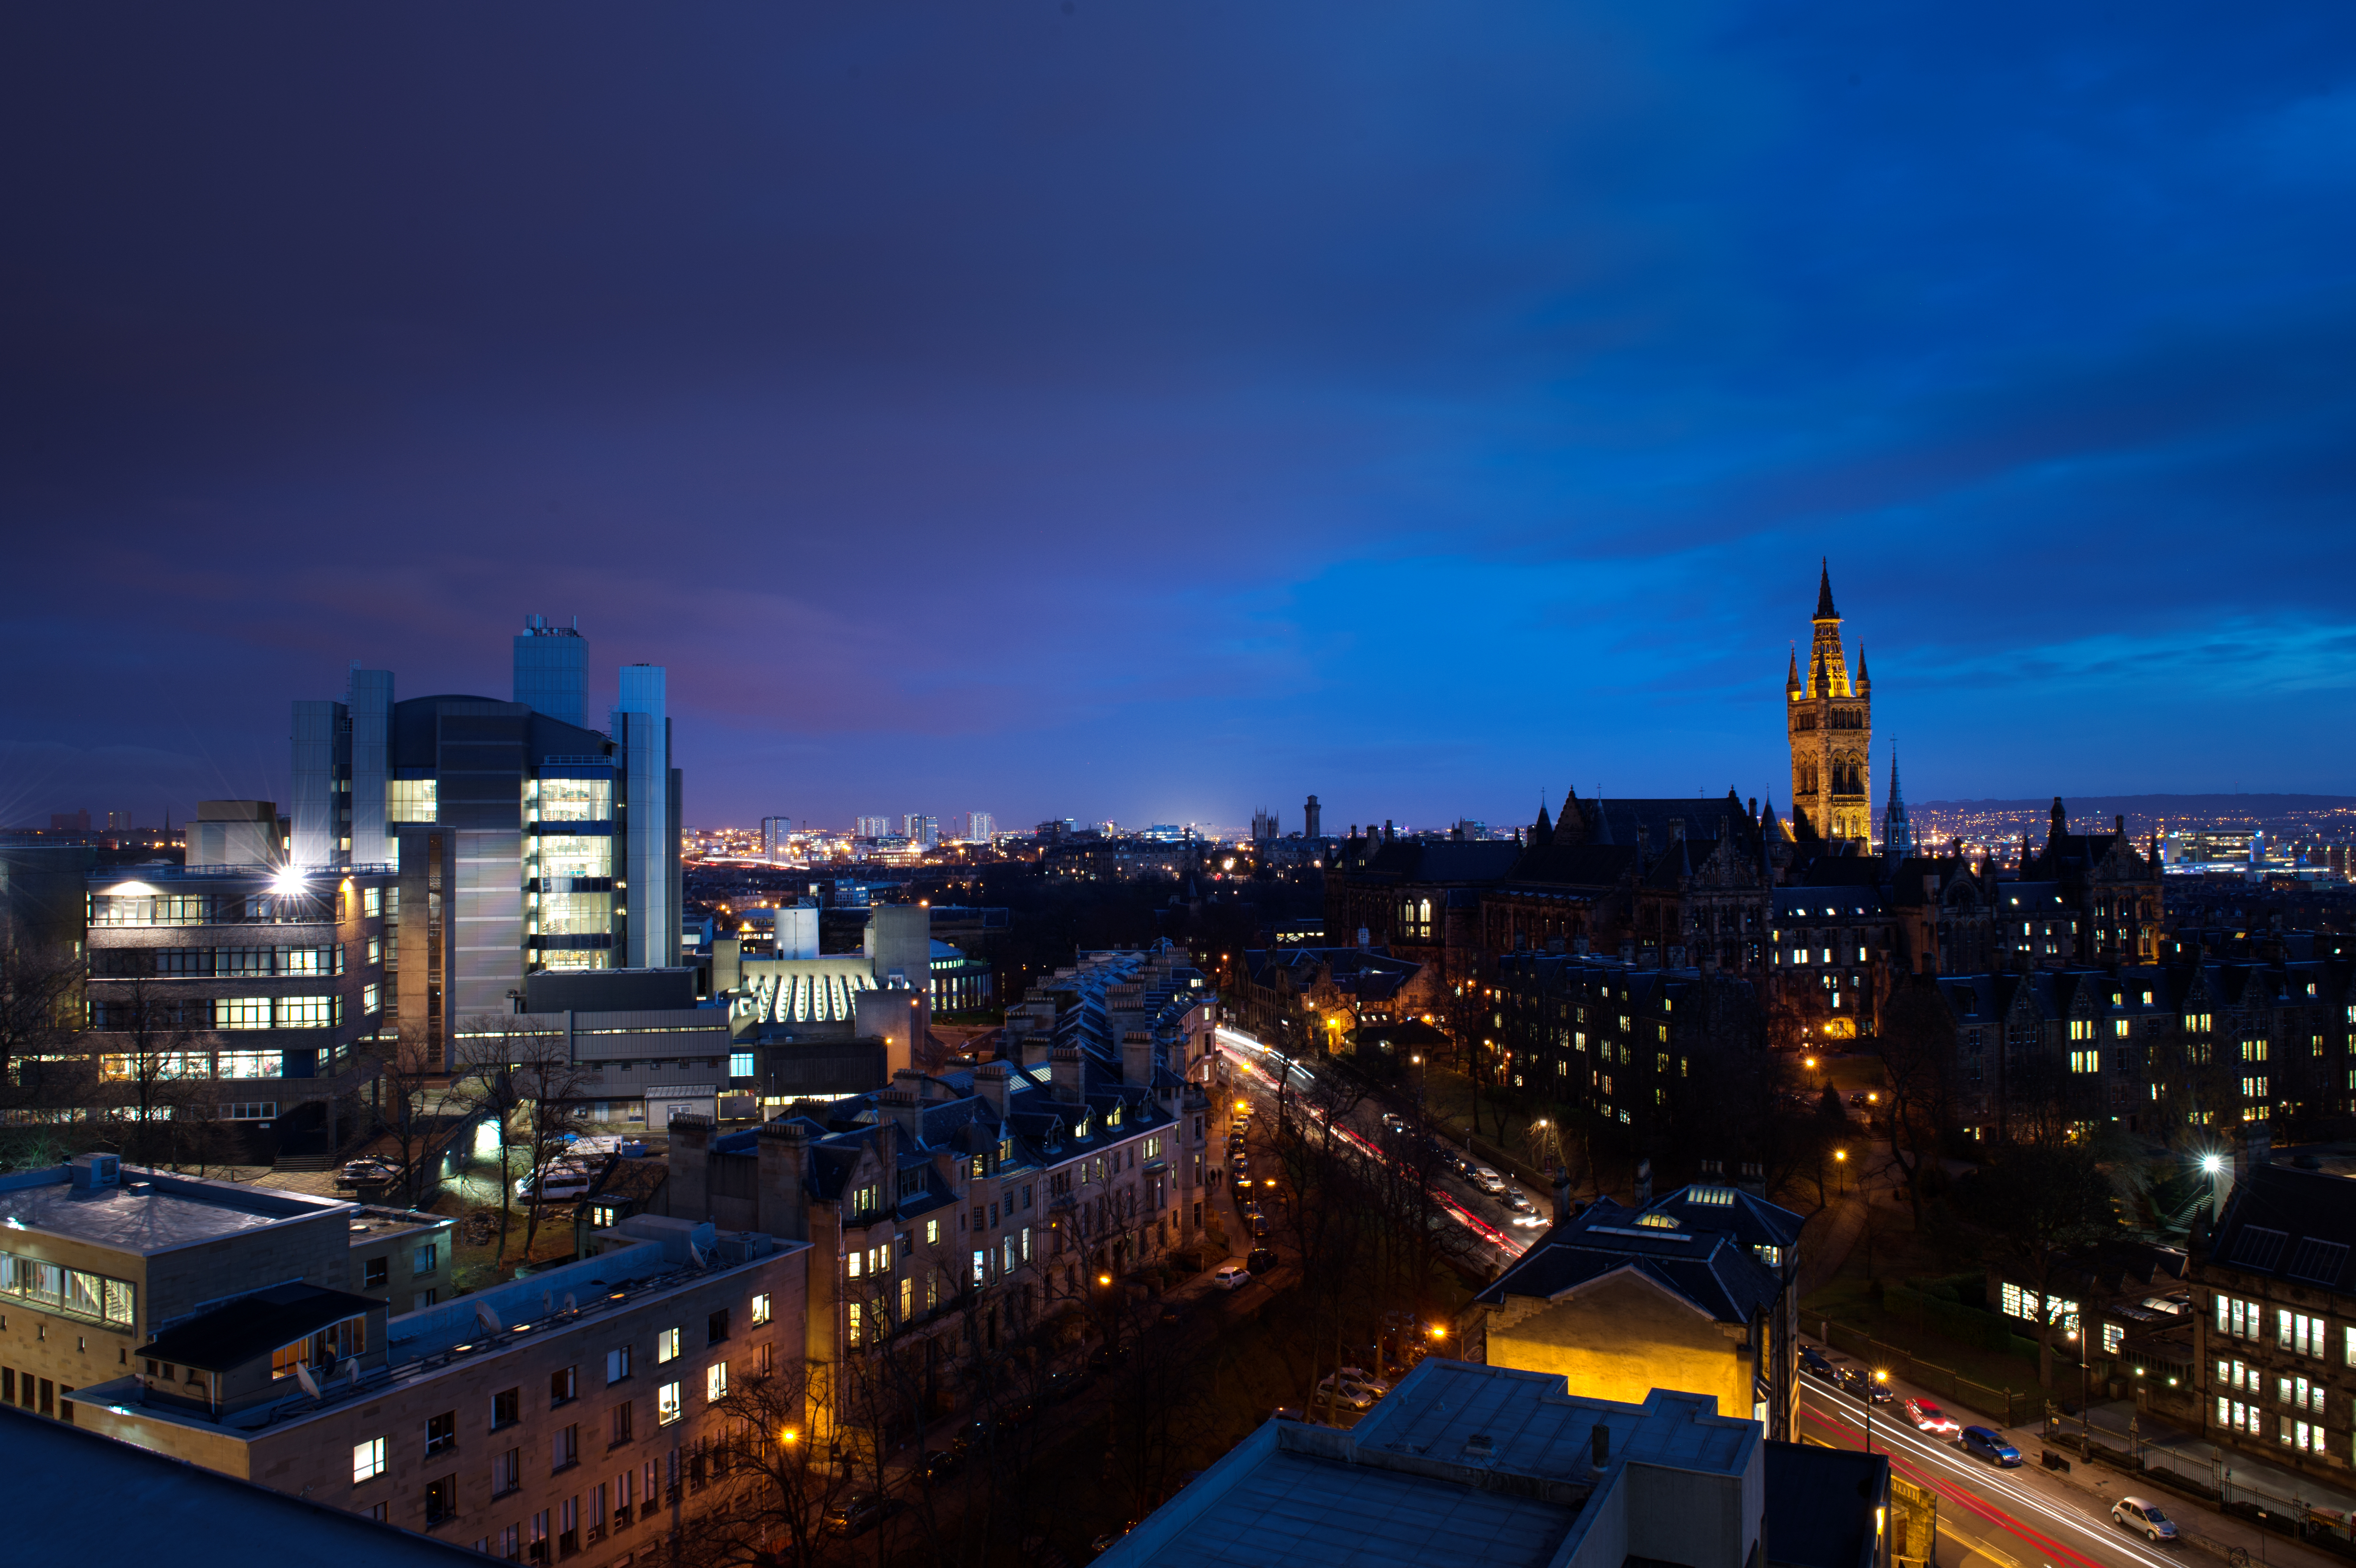
\includegraphics[keepaspectratio=true, width=\paperwidth]{../../images/background2.jpg}};
    }

    \begin{frame}[plain,noframenumbering]
        \begin{tikzpicture}[remember picture, overlay]
            \node at (current page.north west) {
                \begin{tikzpicture}[remember picture, overlay]
                    \fill [fill=uofguniversityblue, anchor=north west] (0, 0) rectangle (\paperwidth, -2.8cm);
                \end{tikzpicture}
            };

            \node (logo) [anchor=north east, shift={(-0.8cm,-0.2cm)}] at (current page.north east) {
                \includegraphics[keepaspectratio=true,scale=0.5]{../../images/UoG_keyline.pdf}
            };

            \node (logo2) [anchor=north, below=0.2cm of logo.south] {
                \includegraphics[keepaspectratio=true,scale=0.1]{../../images/RAEngWhite.pdf}
            };

            \coordinate (logos) at ($(logo.south)!0.5!(logo2.north)$);

            \node [anchor=west, xshift=0.8cm] at (current page.west |- logos) {
                \begin{minipage}{0.60\paperwidth}\raggedright
                    \textcolor{white}{\url{https://ciaranm.github.io/}} \\[0.3cm]
                    \textcolor{white}{\href{mailto:ciaran.mccreesh@glasgow.ac.uk}{\nolinkurl{ciaran.mccreesh@glasgow.ac.uk}}}
                \end{minipage}
            };
            \node [anchor=south, yshift=0.3cm, rounded corners, fill opacity=0.9, fill=white, draw] at (current page.south) {
                \begin{minipage}{0.6\paperwidth}
                    \centering
                \large Hiring for a 3yr postdoc position. \\
                    See \url{https://ciaranm.github.io/}
                \end{minipage}
            };

        \end{tikzpicture}
    \end{frame}
}

\end{document}

